\section{System Architecture Diagrams}

This appendix contains the complete set of technical diagrams, system architecture illustrations, and visual documentation supporting the Multi-Sensor Recording System thesis. These diagrams provide detailed visual representations of system components, data flows, and architectural relationships.

\subsection{High-Level System Architecture}

\subsubsection{Overall System Architecture}

\begin{figure}[htbp]
\centering
\begin{tikzpicture}[
    node distance=2cm,
    component/.style={rectangle, draw=blue!60, fill=blue!5, thick, minimum width=3cm, minimum height=1.5cm, text centered},
    device/.style={rectangle, draw=green!60, fill=green!5, thick, minimum width=2.5cm, minimum height=1cm, text centered},
    sensor/.style={rectangle, draw=red!60, fill=red!5, thick, minimum width=2cm, minimum height=0.8cm, text centered},
    connection/.style={thick, ->}
]

% Desktop Controller
\node[component] (controller) {Desktop Controller\\(Python)};

% Network Layer
\node[component, below=1cm of controller] (network) {Network Communication Layer\\(WebSocket/TCP)};

% Android Devices
\node[device, below left=2cm and 2cm of network] (android1) {Android Device 1\\(Sensor Node)};
\node[device, below=2cm of network] (android2) {Android Device 2\\(Sensor Node)};
\node[device, below right=2cm and 2cm of network] (android3) {Android Device 3\\(Sensor Node)};

% Sensors
\node[sensor, below=1cm of android1] (thermal1) {Thermal\\Camera};
\node[sensor, below=1cm of android2] (thermal2) {Thermal\\Camera};
\node[sensor, below=1cm of android3] (shimmer1) {Shimmer\\GSR};

% Data Storage
\node[component, right=3cm of controller] (storage) {Data Storage\\\& Management};

% Connections
\draw[connection] (controller) -- (network);
\draw[connection] (network) -- (android1);
\draw[connection] (network) -- (android2);
\draw[connection] (network) -- (android3);
\draw[connection] (android1) -- (thermal1);
\draw[connection] (android2) -- (thermal2);
\draw[connection] (android3) -- (shimmer1);
\draw[connection] (controller) -- (storage);

% Network annotations
\node[above=0.3cm of network, text width=4cm, text centered] {5GHz WiFi Network\\mDNS Discovery\\NTP Synchronization};

\end{tikzpicture}
\caption{Multi-Sensor Recording System Architecture Overview}
\label{fig:system_architecture_overview}
\end{figure}

Figure~\ref{fig:system_architecture_overview} illustrates the distributed architecture of the Multi-Sensor Recording System, showing the central desktop controller coordinating multiple Android sensor nodes through a network communication layer.

\subsection{Component Integration Diagrams}

\subsubsection{Android Application Architecture}

\begin{figure}[htbp]
\centering
\begin{tikzpicture}[
    node distance=1.5cm,
    layer/.style={rectangle, draw=black, thick, minimum width=8cm, minimum height=1.2cm, text centered},
    component/.style={rectangle, draw=blue!60, fill=blue!10, thick, minimum width=2.5cm, minimum height=0.8cm, text centered, font=\small},
    manager/.style={rectangle, draw=green!60, fill=green!10, thick, minimum width=2cm, minimum height=0.8cm, text centered, font=\small}
]

% Application Layers
\node[layer] (ui) {User Interface Layer};
\node[layer, below=0.2cm of ui] (control) {Recording Control Layer};
\node[layer, below=0.2cm of control] (sensor) {Sensor Management Layer};
\node[layer, below=0.2cm of sensor] (comm) {Communication Layer};
\node[layer, below=0.2cm of comm] (hw) {Hardware Abstraction Layer};

% Components in each layer
\node[component, above=1.5cm of ui] (session) {Session\\Manager};
\node[component, left=1cm of session] (preview) {Live\\Preview};
\node[component, right=1cm of session] (status) {Status\\Monitor};

\node[manager, above=1.5cm of control] (rgb) {RGB Camera\\Manager};
\node[manager, left=1cm of rgb] (thermal) {Thermal\\Manager};
\node[manager, right=1cm of rgb] (gsr) {GSR Sensor\\Manager};

\node[component, above=1.5cm of sensor] (sync) {Time Sync\\Service};
\node[component, left=1cm of sync] (data) {Data\\Logger};
\node[component, right=1cm of sync] (network) {Network\\Client};

% Hardware interfaces
\node[manager, above=1.5cm of hw] (camerax) {CameraX\\API};
\node[manager, left=1cm of camerax] (uvc) {UVC\\Camera};
\node[manager, right=1cm of camerax] (ble) {BLE\\Stack};

\end{tikzpicture}
\caption{Android Application Layered Architecture}
\label{fig:android_architecture}
\end{figure}

\subsubsection{Desktop Controller Architecture}

\begin{figure}[htbp]
\centering
\begin{tikzpicture}[
    node distance=2cm,
    module/.style={rectangle, draw=blue!60, fill=blue!10, thick, minimum width=2.5cm, minimum height=1.5cm, text centered},
    service/.style={rectangle, draw=green!60, fill=green!10, thick, minimum width=2cm, minimum height=1cm, text centered},
    interface/.style={rectangle, draw=purple!60, fill=purple!10, thick, minimum width=2cm, minimum height=1cm, text centered}
]

% Main modules
\node[module] (gui) {PyQt6\\GUI};
\node[module, below=1cm of gui] (session) {Session\\Controller};
\node[module, left=2cm of session] (device) {Device\\Manager};
\node[module, right=2cm of session] (data) {Data\\Manager};

% Services
\node[service, below=1cm of device] (discovery) {Device\\Discovery};
\node[service, below=1cm of session] (sync) {Time Sync\\Server};
\node[service, below=1cm of data] (validation) {Data\\Validation};

% Interfaces
\node[interface, below=1cm of discovery] (network) {Network\\Interface};
\node[interface, below=1cm of sync] (storage) {Storage\\Interface};
\node[interface, below=1cm of validation] (export) {Export\\Interface};

% Connections
\draw[thick, ->] (gui) -- (session);
\draw[thick, ->] (session) -- (device);
\draw[thick, ->] (session) -- (data);
\draw[thick, ->] (device) -- (discovery);
\draw[thick, ->] (session) -- (sync);
\draw[thick, ->] (data) -- (validation);
\draw[thick, ->] (discovery) -- (network);
\draw[thick, ->] (sync) -- (storage);
\draw[thick, ->] (validation) -- (export);

\end{tikzpicture}
\caption{Desktop Controller Modular Architecture}
\label{fig:desktop_architecture}
\end{figure>

\section{Data Flow Diagrams}

\subsection{Multi-Modal Data Collection Flow}

\begin{figure}[htbp]
\centering
\begin{tikzpicture}[
    node distance=2cm,
    source/.style={ellipse, draw=red!60, fill=red!10, thick, minimum width=2cm, minimum height=1cm, text centered},
    process/.style={rectangle, draw=blue!60, fill=blue!10, thick, minimum width=2.5cm, minimum height=1cm, text centered},
    store/.style={rectangle, draw=green!60, fill=green!10, thick, minimum width=2cm, minimum height=1cm, text centered},
    flow/.style={thick, ->}
]

% Data sources
\node[source] (participant) {Participant};
\node[source, below=1cm of participant] (stimuli) {Stimuli\\Events};

% Sensors
\node[process, right=3cm of participant] (gsr_sensor) {GSR\\Sensor};
\node[process, above=1cm of gsr_sensor] (thermal_cam) {Thermal\\Camera};
\node[process, below=1cm of gsr_sensor] (rgb_cam) {RGB\\Camera};

% Processing
\node[process, right=3cm of gsr_sensor] (timestamp) {Timestamp\\Sync};
\node[process, above=1cm of timestamp] (thermal_proc) {Thermal\\Processing};
\node[process, below=1cm of timestamp] (video_proc) {Video\\Processing};

% Storage
\node[store, right=3cm of timestamp] (csv_store) {CSV\\Files};
\node[store, above=1cm of csv_store] (thermal_store) {Thermal\\Data};
\node[store, below=1cm of csv_store] (video_store) {Video\\Files};

% Final output
\node[store, right=2cm of csv_store] (dataset) {Synchronized\\Dataset};

% Flows
\draw[flow] (participant) -- (gsr_sensor);
\draw[flow] (participant) -- (thermal_cam);
\draw[flow] (participant) -- (rgb_cam);
\draw[flow] (stimuli) -- (gsr_sensor);
\draw[flow] (stimuli) -- (thermal_cam);
\draw[flow] (stimuli) -- (rgb_cam);

\draw[flow] (gsr_sensor) -- (timestamp);
\draw[flow] (thermal_cam) -- (thermal_proc);
\draw[flow] (rgb_cam) -- (video_proc);

\draw[flow] (timestamp) -- (csv_store);
\draw[flow] (thermal_proc) -- (thermal_store);
\draw[flow] (video_proc) -- (video_store);

\draw[flow] (csv_store) -- (dataset);
\draw[flow] (thermal_store) -- (dataset);
\draw[flow] (video_store) -- (dataset);

\end{tikzpicture}
\caption{Multi-Modal Data Collection Flow}
\label{fig:data_collection_flow}
\end{figure}

\subsection{Synchronization Protocol Flow}

\begin{figure}[htbp]
\centering
\begin{tikzpicture}[
    node distance=1cm,
    entity/.style={rectangle, draw=black, thick, minimum width=3cm, minimum height=0.8cm, text centered},
    message/.style={thick, ->},
    time/.style={dashed, gray}
]

% Entities
\node[entity] (controller) {Desktop Controller};
\node[entity, right=6cm of controller] (device1) {Android Device 1};
\node[entity, right=3cm of device1] (device2) {Android Device 2};

% Timeline
\draw[time] ([yshift=-0.5cm]controller.south) -- ([yshift=-12cm]controller.south);
\draw[time] ([yshift=-0.5cm]device1.south) -- ([yshift=-12cm]device1.south);
\draw[time] ([yshift=-0.5cm]device2.south) -- ([yshift=-12cm]device2.south);

% Messages
\draw[message] ([yshift=-1cm]controller.south) -- ([yshift=-1cm]device1.south) node[midway, above] {TIME\_SYNC\_REQ};
\draw[message] ([yshift=-1cm]controller.south) -- ([yshift=-1cm]device2.south) node[midway, above] {TIME\_SYNC\_REQ};

\draw[message] ([yshift=-2cm]device1.south) -- ([yshift=-2cm]controller.south) node[midway, above] {TIME\_SYNC\_RESP};
\draw[message] ([yshift=-2cm]device2.south) -- ([yshift=-2cm]controller.south) node[midway, above] {TIME\_SYNC\_RESP};

\draw[message] ([yshift=-4cm]controller.south) -- ([yshift=-4cm]device1.south) node[midway, above] {SESSION\_START};
\draw[message] ([yshift=-4cm]controller.south) -- ([yshift=-4cm]device2.south) node[midway, above] {SESSION\_START};

% Synchronized recording period
\fill[blue!20, opacity=0.3] ([xshift=-1.5cm, yshift=-5cm]controller.south) rectangle ([xshift=1.5cm, yshift=-9cm]device2.south);
\node[above] at ([yshift=-5cm]device1.south) {Synchronized Recording};

\draw[message] ([yshift=-10cm]controller.south) -- ([yshift=-10cm]device1.south) node[midway, above] {SESSION\_STOP};
\draw[message] ([yshift=-10cm]controller.south) -- ([yshift=-10cm]device2.south) node[midway, above] {SESSION\_STOP};

\end{tikzpicture}
\caption{Synchronization Protocol Message Flow}
\label{fig:sync_protocol_flow}
\end{figure}

\section{User Interface Diagrams}

\subsection{Desktop Application GUI Layout}

\begin{figure}[htbp]
\centering
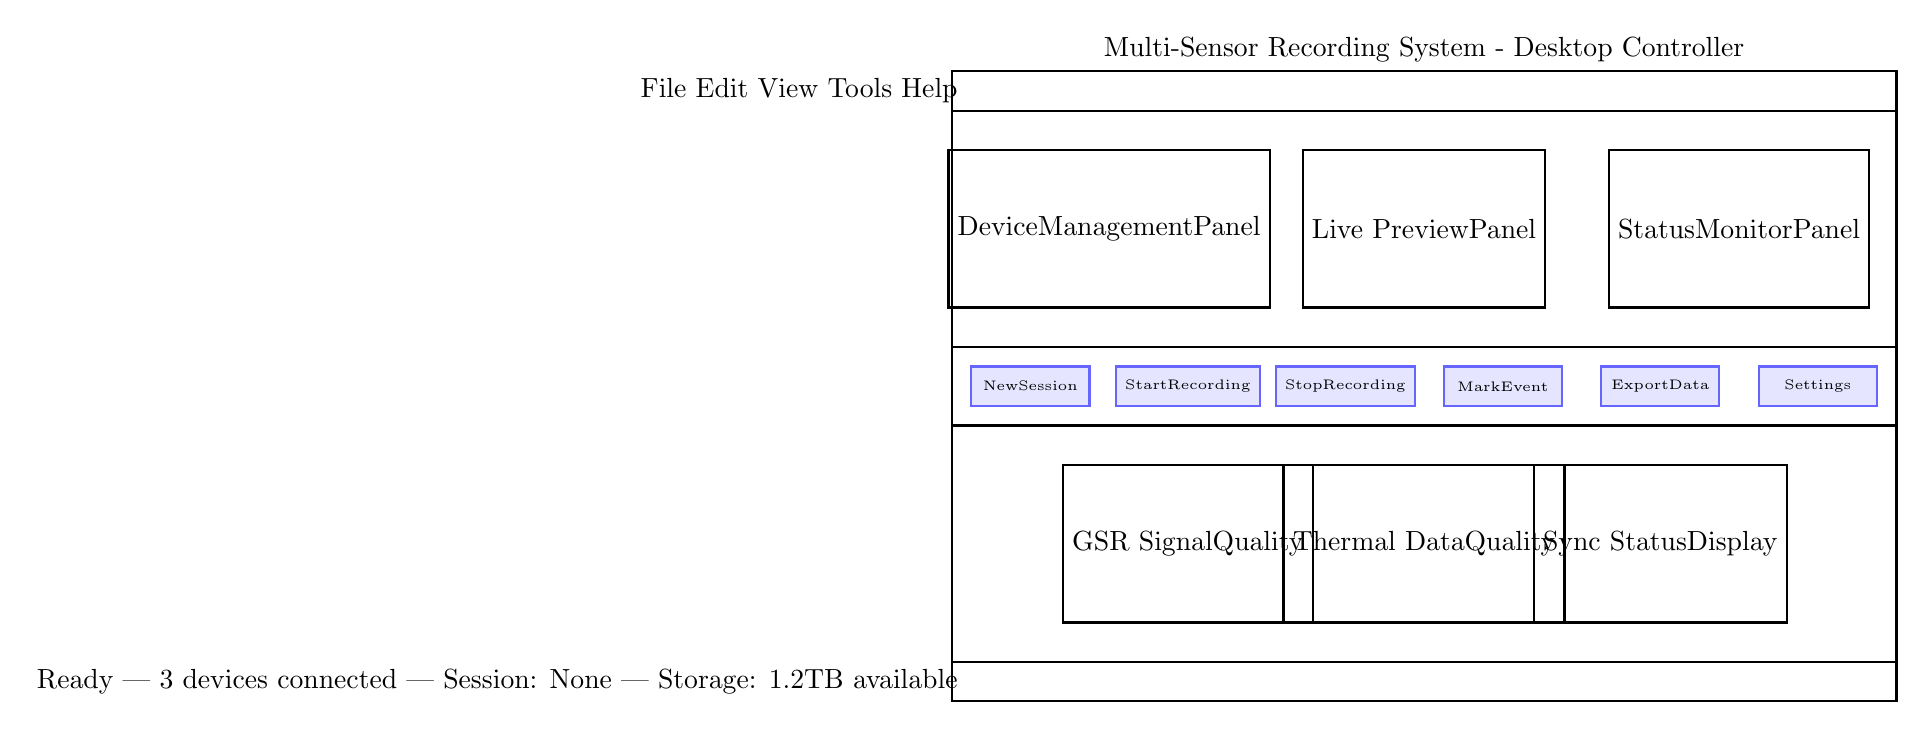
\begin{tikzpicture}[
    node distance=0.1cm,
    panel/.style={rectangle, draw=black, thick, minimum width=3cm, minimum height=2cm, text centered},
    button/.style={rectangle, draw=blue!60, fill=blue!10, thick, minimum width=1.5cm, minimum height=0.5cm, text centered, font=\tiny},
    display/.style={rectangle, draw=green!60, fill=green!10, thick, minimum width=2cm, minimum height=1cm, text centered, font=\tiny}
]

% Main window frame
\draw[thick] (0,0) rectangle (12,8);
\node[above] at (6,8) {Multi-Sensor Recording System - Desktop Controller};

% Menu bar
\draw[thick] (0,7.5) rectangle (12,8);
\node[left] at (0.2,7.75) {File Edit View Tools Help};

% Main panels
\node[panel] at (2,6) {Device\\Management\\Panel};
\node[panel] at (6,6) {Live Preview\\Panel};
\node[panel] at (10,6) {Status\\Monitor\\Panel};

% Control panel
\draw[thick] (0,3.5) rectangle (12,4.5);
\node[button] at (1,4) {New\\Session};
\node[button] at (3,4) {Start\\Recording};
\node[button] at (5,4) {Stop\\Recording};
\node[button] at (7,4) {Mark\\Event};
\node[button] at (9,4) {Export\\Data};
\node[button] at (11,4) {Settings};

% Data quality panel
\node[panel] at (3,2) {GSR Signal\\Quality};
\node[panel] at (6,2) {Thermal Data\\Quality};
\node[panel] at (9,2) {Sync Status\\Display};

% Status bar
\draw[thick] (0,0) rectangle (12,0.5);
\node[left] at (0.2,0.25) {Ready | 3 devices connected | Session: None | Storage: 1.2TB available};

\end{tikzpicture}
\caption{Desktop Controller GUI Layout}
\label{fig:desktop_gui_layout}
\end{figure}

\subsection{Android Application Interface}

\begin{figure}[htbp]
\centering
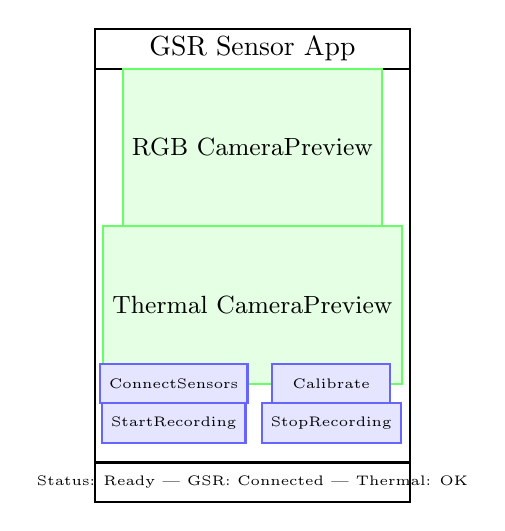
\begin{tikzpicture}[
    node distance=0.1cm,
    screen/.style={rectangle, draw=black, thick, minimum width=4cm, minimum height=6cm},
    widget/.style={rectangle, draw=blue!60, fill=blue!10, thick, minimum width=1.5cm, minimum height=0.5cm, text centered, font=\tiny},
    preview/.style={rectangle, draw=green!60, fill=green!10, thick, minimum width=3cm, minimum height=2cm, text centered, font=\small}
]

% Phone screen
\draw[thick] (0,0) rectangle (4,6);

% Title bar
\draw[thick] (0,5.5) rectangle (4,6);
\node at (2,5.75) {GSR Sensor App};

% Camera previews
\node[preview] at (2,4.5) {RGB Camera\\Preview};
\node[preview] at (2,2.5) {Thermal Camera\\Preview};

% Control buttons
\node[widget] at (1,1.5) {Connect\\Sensors};
\node[widget] at (3,1.5) {Calibrate};
\node[widget] at (1,1) {Start\\Recording};
\node[widget] at (3,1) {Stop\\Recording};

% Status indicators
\draw[thick] (0,0) rectangle (4,0.5);
\node[font=\tiny] at (2,0.25) {Status: Ready | GSR: Connected | Thermal: OK};

\end{tikzpicture}
\caption{Android Application Interface Layout}
\label{fig:android_gui_layout}
\end{figure}

\section{Network and Communication Diagrams}

\subsection{Network Topology}

\begin{figure}[htbp]
\centering
\begin{tikzpicture}[
    node distance=2cm,
    controller/.style={rectangle, draw=blue!60, fill=blue!10, thick, minimum width=2.5cm, minimum height=1.5cm, text centered},
    device/.style={rectangle, draw=green!60, fill=green!10, thick, minimum width=2cm, minimum height=1cm, text centered},
    network/.style={ellipse, draw=red!60, fill=red!10, thick, minimum width=3cm, minimum height=1.5cm, text centered},
    connection/.style={thick}
]

% Network hub
\node[network] (wifi) {5GHz WiFi\\Network\\Router};

% Desktop controller
\node[controller, above=2cm of wifi] (desktop) {Desktop\\Controller\\192.168.1.10};

% Android devices
\node[device, left=2.5cm of wifi] (android1) {Android 1\\192.168.1.101};
\node[device, right=2.5cm of wifi] (android2) {Android 2\\192.168.1.102};
\node[device, below left=2cm and 1cm of wifi] (android3) {Android 3\\192.168.1.103};
\node[device, below right=2cm and 1cm of wifi] (android4) {Android 4\\192.168.1.104};

% Connections
\draw[connection] (desktop) -- (wifi);
\draw[connection] (android1) -- (wifi);
\draw[connection] (android2) -- (wifi);
\draw[connection] (android3) -- (wifi);
\draw[connection] (android4) -- (wifi);

% Port annotations
\node[font=\tiny, above left] at ([xshift=-0.5cm, yshift=0.5cm]wifi.center) {TCP 8080\\TCP 8081\\UDP 5353};

\end{tikzpicture}
\caption{System Network Topology}
\label{fig:network_topology}
\end{figure>

\subsection{Protocol Stack}

\begin{figure}[htbp]
\centering
\begin{tikzpicture}[
    node distance=0.1cm,
    layer/.style={rectangle, draw=black, thick, minimum width=8cm, minimum height=1cm, text centered}
]

% Protocol layers
\node[layer, fill=blue!20] (app) {Application Layer: Session Control, Data Streaming, Device Management};
\node[layer, fill=green!20, below=0.05cm of app] (presentation) {Presentation Layer: JSON Serialization, Data Compression};
\node[layer, fill=yellow!20, below=0.05cm of presentation] (session) {Session Layer: WebSocket Connections, Authentication};
\node[layer, fill=orange!20, below=0.05cm of session] (transport) {Transport Layer: TCP (Control), UDP (Discovery)};
\node[layer, fill=red!20, below=0.05cm of transport] (network) {Network Layer: IPv4, mDNS, NTP};
\node[layer, fill=purple!20, below=0.05cm of network] (datalink) {Data Link Layer: Ethernet, WiFi 802.11ac};
\node[layer, fill=gray!20, below=0.05cm of datalink] (physical) {Physical Layer: 5GHz Radio, Ethernet Cable};

\end{tikzpicture}
\caption{Communication Protocol Stack}
\label{fig:protocol_stack}
\end{figure>

\section{Data Model Diagrams}

\subsection{Database Schema}

\begin{figure}[htbp]
\centering
\begin{tikzpicture}[
    node distance=2cm,
    table/.style={rectangle, draw=black, thick, minimum width=3cm, text centered},
    field/.style={rectangle, draw=gray, minimum width=2.8cm, text left, font=\tiny},
    relation/.style={thick, ->}
]

% Sessions table
\node[table] (sessions) {Sessions};
\node[field, below=0.1cm of sessions] (s1) {session\_id (PK)};
\node[field, below=0.05cm of s1] (s2) {participant\_id};
\node[field, below=0.05cm of s2] (s3) {start\_time};
\node[field, below=0.05cm of s3] (s4) {end\_time};
\node[field, below=0.05cm of s4] (s5) {status};

% Devices table
\node[table, right=3cm of sessions] (devices) {Devices};
\node[field, below=0.1cm of devices] (d1) {device\_id (PK)};
\node[field, below=0.05cm of d1] (d2) {session\_id (FK)};
\node[field, below=0.05cm of d2] (d3) {device\_type};
\node[field, below=0.05cm of d3] (d4) {capabilities};

% GSR Data table
\node[table, below=2cm of sessions] (gsr) {GSR\_Data};
\node[field, below=0.1cm of gsr] (g1) {timestamp (PK)};
\node[field, below=0.05cm of g1] (g2) {session\_id (FK)};
\node[field, below=0.05cm of g2] (g3) {gsr\_value};
\node[field, below=0.05cm of g3] (g4) {temperature};

% Thermal Data table
\node[table, below=2cm of devices] (thermal) {Thermal\_Data};
\node[field, below=0.1cm of thermal] (t1) {timestamp (PK)};
\node[field, below=0.05cm of t1] (t2) {session\_id (FK)};
\node[field, below=0.05cm of t2] (t3) {frame\_id};
\node[field, below=0.05cm of t3] (t4) {pixel\_data};

% Relations
\draw[relation] (sessions) -- (devices);
\draw[relation] (sessions) -- (gsr);
\draw[relation] (sessions) -- (thermal);

\end{tikzpicture}
\caption{Data Model Schema}
\label{fig:data_model}
\end{figure}

This comprehensive collection of diagrams provides detailed visual documentation of all aspects of the Multi-Sensor Recording System architecture, supporting both technical implementation and research applications.
